\begin{figure}[h!]
\tikzset{every picture/.style={line width=0.75pt}} %set default line width to 0.75pt        
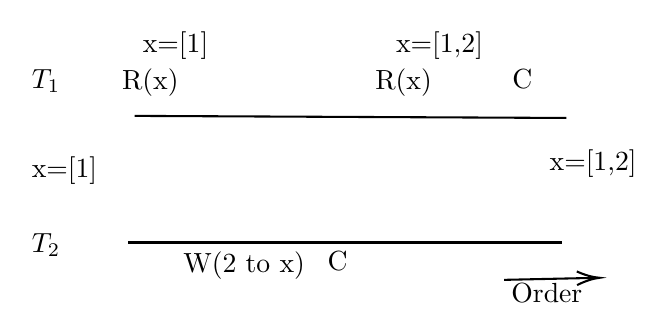
\begin{tikzpicture}[x=0.75pt,y=0.75pt,yscale=-1,xscale=1]
%uncomment if require: \path (0,300); %set diagram left start at 0, and has height of 300

%Straight Lines [id:da9500410641573396] 
\draw    (63.56,64) -- (271.56,65) ;
%Straight Lines [id:da7796185686481738] 
\draw    (60.56,125) -- (269.56,125) ;
%Straight Lines [id:da7329480179958066] 
\draw    (241.56,143) -- (285.56,142.04) ;
\draw [shift={(287.56,142)}, rotate = 178.75] [color={rgb, 255:red, 0; green, 0; blue, 0 }  ][line width=0.75]    (10.93,-3.29) .. controls (6.95,-1.4) and (3.31,-0.3) .. (0,0) .. controls (3.31,0.3) and (6.95,1.4) .. (10.93,3.29)   ;

% Text Node
\draw (12.5,40) node [anchor=north west][inner sep=0.75pt]   [align=left] {$T_1$};
% Text Node
\draw (12.5,119) node [anchor=north west][inner sep=0.75pt]   [align=left] {$T_2$};
% Text Node
\draw (85.56,128) node [anchor=north west][inner sep=0.75pt]   [align=left] {W(2 to x)};
% Text Node
\draw (56,40) node [anchor=north west][inner sep=0.75pt]   [align=left] {R(x)};
% Text Node
\draw (244,40) node [anchor=north west][inner sep=0.75pt]   [align=left] {C};
% Text Node
\draw (155,128) node [anchor=north west][inner sep=0.75pt]   [align=left] {C};
% Text Node
\draw (243.56,143) node [anchor=north west][inner sep=0.75pt]   [align=left] {Order};
% Text Node
\draw (12.5,82) node [anchor=north west][inner sep=0.75pt]   [align=left] {x=[1]};
% Text Node
\draw (66,22) node [anchor=north west][inner sep=0.75pt]   [align=left] {x=[1]};
% Text Node
\draw (178,40) node [anchor=north west][inner sep=0.75pt]   [align=left] {R(x)};
% Text Node
\draw (188,22) node [anchor=north west][inner sep=0.75pt]   [align=left] {x=[1,2]};
% Text Node
\draw (262,79) node [anchor=north west][inner sep=0.75pt]   [align=left] {x=[1,2]};
\end{tikzpicture}
\caption{P2: Non-repeatable/Fuzzy Read between $T_1$ and $T_2$}
\end{figure}